\section{Nodes}
Our weather station's primary components are the nodes, which gather weather data through various sensors. We have selected three specific sensors: temperature, humidity, and pressure.\\
To achieve this, we have employed two Arduino Nano devices situated in different locations. Each Arduino Nano is equipped with temperature, pressure, \& humidity sensors. \\ Through LoRa communication, the collected data is transmitted to the central system, where it undergoes processing and storage for future utilization. Access to the accumulated data is facilitated through the website.


\textcolor{red}{Keep in mind:}
Our project is mainly the central part of the weather station, so this section won't go into detail as the Central section.

\subsection{Choice of parts \& material}

\subsubsection{Arduino}
For the Arduino, we don't really need anything fancy, a simple Arduino Nano will be more than sufficient.
\begin{table}[H]
    \centering
    \begin{tabular}{|l|l|}
        \hline
        \textbf{MCU} & \textbf{ATmega328P} \\ \hline
        Architecture & AVR \\ \hline
        Operating Voltage & 5V \\ \hline
        Input Voltage & 7V - 12V \\ \hline
        Clock Speed & 16 MHz \\ \hline
        Flash Memory & 32 KB (2 KB used by bootloader) \\ \hline
        SRAM & 2 KB \\ \hline
        EEPROM & 1 KB \\ \hline
        Digital IO Pins & 22 (6 PWM) \\ \hline
        Analog Input Pins & 8 \\ \hline
    \end{tabular}
    \caption{Arduino Nano Specs}
\end{table}

\subsubsection{LoRa Module}
We chose \verb|Grove - Long Range 868MHz| because of its capabilities and ease of use.
 \begin{itemize}
    \item Using RFM95 module based on SX1276 LoRa®
    \item Working Voltage: 5V/3.3V
    \item ~28mA(Avg) @+20dBm continuous transmit
    \item ~8.4mA(Avg) @standby mode
    \item ~20mA(Avg) @receive mode, BW-500kHz
    \item Working Temperature: -20 – 70℃
    \item Interface: Grove - UART (RX, TX, VCC, GND)
    \item Simple wire antenna or MHF Connector for external high gain antenna
    \item Working Frequency: 868MHz/433MHz
    \item +20dBm 100 mW Power Output Capability
    \item Size: 20*40mm
    \item Rate: 0.3kps \~ 50kps
    \item Ready-to-go Arduino libraries
    \item Reserved MHF antenna connector
\end{itemize}
\begin{table}[H]
    \caption{Grove - Long Range 868MHz Specs \& Features}
\end{table}
The module already provides an Arduino Library to interface with it through Serial communication.
\begin{figure}[H]
    \centering
    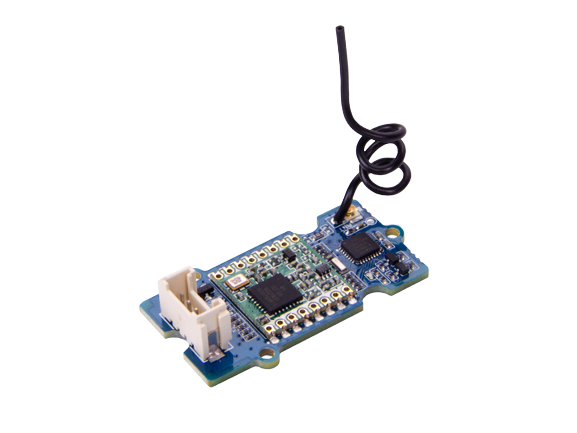
\includegraphics[width=.6\textwidth]{images/node/grove_lora.png}
    \caption{Grove - Long Range 868MHz (LoRa module)}
\end{figure}

\subsubsection{Humidity and Temperature module}
We chose \verb|DHT11| as a temperature and humidity sensor. it is cheap and very easy to interface with requiring only one data line.

\begin{itemize}
    \item Operating Voltage: 3.5V to 5.5V
    \item Operating current: 0.3mA (measuring), 60uA (standby)
    \item Output: Serial data
    \item Temperature Range: 0°C to 50°C
    \item Humidity Range: 20\% to 90\%
    \item Resolution: Temperature and Humidity both are 16-bit
    \item Accuracy: ±1°C and ±1\%
\end{itemize}
\begin{table}[H]
    \caption{DHT11 Specs \& Features}
\end{table}
\begin{figure}[H]
    \centering
    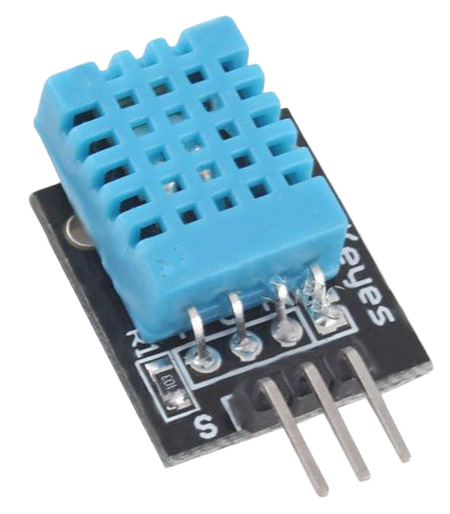
\includegraphics[width=.4\textwidth]{images/node/dht11.png}
    \caption{DHT 11}
\end{figure}

\subsubsection{Pressure Sensor}
We used \verb|BMP388| as a pressure sensor, it also measures the temperature, but we won't be using it since we already have the \verb|DHT11|.

\begin{table}[H]
    \centering
    \begin{tabular}{|p{8cm}|p{6cm}|}
        \hline
        \textbf{Parameter} & \textbf{Value} \\ \hline
        Operation range (Pressure) & 300...1250 hPa \\ \hline
        Supply voltage (VDDIO) & 1.2 V...3.6 V \\ \hline
        Supply voltage (VDD) & 1.65 V...3.6 V \\ \hline
        Interface & I²C and SPI \\ \hline
        Average typical current consumption (1 Hz data rate) & 3.4 µA @ 1Hz \\ \hline
        Absolute accuracy pressure (typ.) & P=900...1100 hPa (T=25...40°C) \& ±0.5 hPa \\ \hline
        Relative accuracy pressure (typ.) & P=900...1100 hPa (T=25...40°C) \& ±0.08 hPa \\ \hline
        Noise in pressure (lowest bandwidth, highest resolution) & 0.03 Pa \\ \hline
        Temperature coefficient offset (-20°...65°C @ 700 hPa to 1100 hPa) & ±0.75 Pa/K \\ \hline
        Long-term stability (12 months) & ±0.33 hPa \\ \hline
        Solder drift & < ±1.0 hPa \\ \hline
        Maximum sampling rate & 200 Hz \\ \hline
    \end{tabular}
    \caption{BMP388 Specs}
\end{table}
\begin{figure}[H]
    \centering
    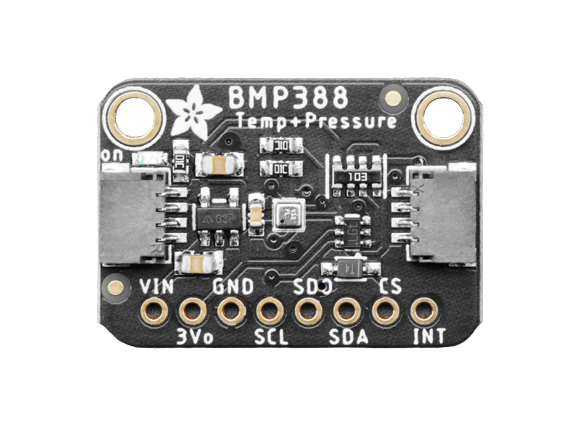
\includegraphics[width=.4\textwidth]{images/node/bmp388.png}
    \caption{DHT 11}
\end{figure}

\subsection{Electrical Schematic}
\begin{figure}[H]
    \centering
    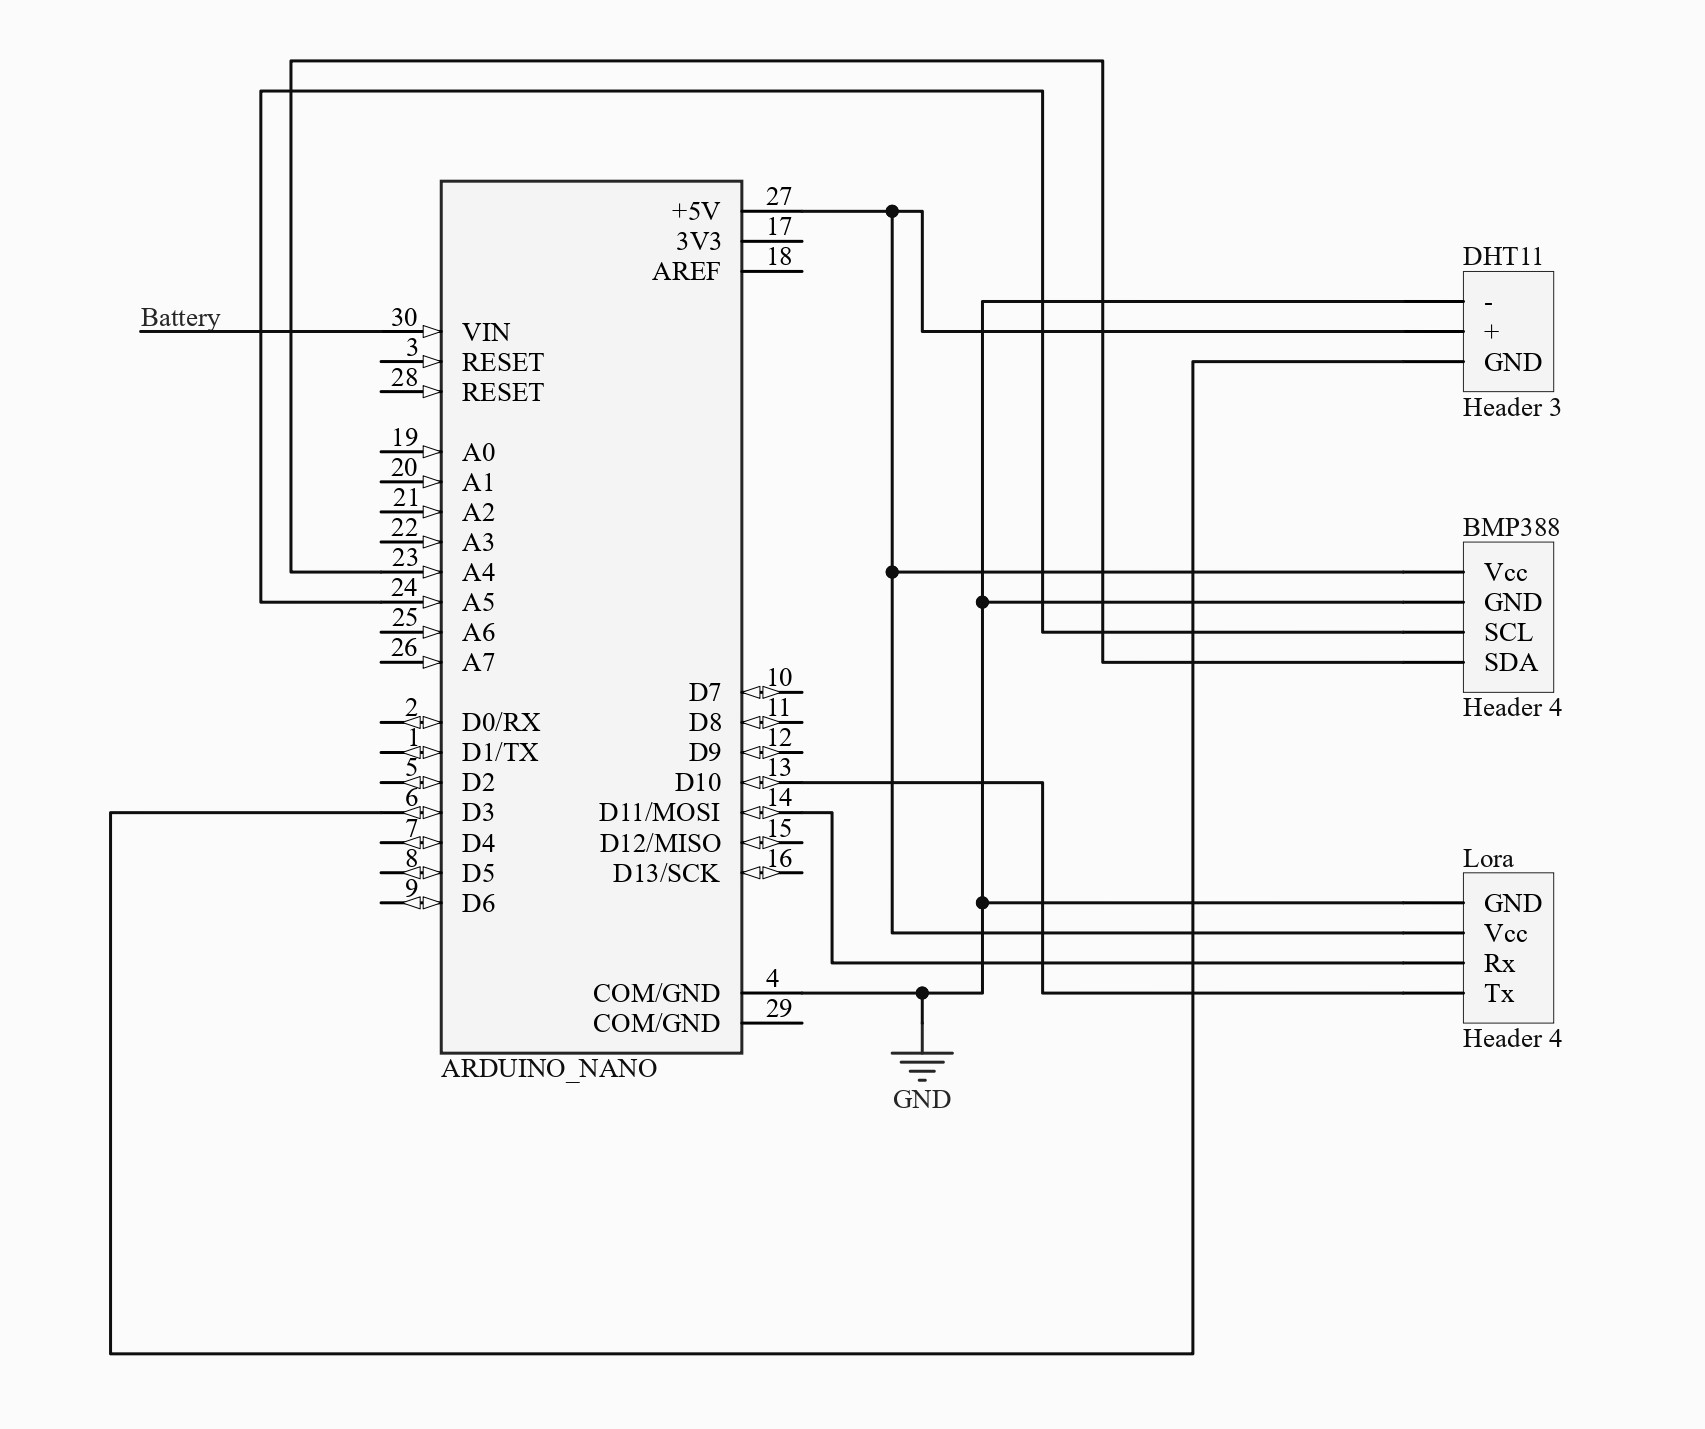
\includegraphics[width=.9\textwidth]{images/VMware Horizon_230508_235208_page-0001.jpg}
    \caption{Node Schematic}
\end{figure}

\subsection{Implementation}

\subsubsection{DHT11}
The module is very simple to interface with using Arduino \& its dedicated library. It is as simple as these for lines to initialize and fetch data.
\begin{code}
    \begin{minted}{c++}
DHT* _module = new DHT(_pin, DHT11);
_module->begin();
    \end{minted}
    \caption{DHT11 initialization}
\end{code}
\begin{code}
    \begin{minted}{c++}
float humidity = _module->readHumidity();
float temperature = _module->readTemperature();
    \end{minted}
    \caption{DHT11 interfacing}
\end{code}

\subsubsection{BMP988}
This module is a bit more verbose than its predecessor, but its library does more of the heavy lifting
\begin{code}
    \begin{minted}{c++}
DFRobot_BMP388_I2C* _module;
BMP388::BMP388()
{
    _module = new DFRobot_BMP388_I2C();
    _module->set_iic_addr(BMP3_I2C_ADDR_PRIM);
}

void BMP388::setup()
{
    Serial.println("Initializing BMP388 (Pressure Sensor)...");
    while (_module->begin() != BMP3_OK)
    {
        Serial.println("BMP388 initialization failed, Retrying...");
        delay(1000);
    }
    Serial.println("BMP388 initialized");
}

void BMP388::run()
{
    float pressure = _module->readPressure();

    float temperature = _module->readTemperature();
}
    \end{minted}
    \caption{BMP388 initiation & interfacing}
\end{code}

\subsubsection{LoRa}
\begin{code}
    \begin{minted}{c++}
Lora::Lora(uint8_t Rx, uint8_t Tx)
{
    _serial = new SoftwareSerial(Rx, Tx);
    _rf95 = new RH_RF95<SoftwareSerial>(*_serial);
}

void Lora::begin(double frequency)
{
    Serial.println("Initializing RF95 (LoRa Module)...");

    while (!_rf95->init())
    {
        Serial.println("RF95 initialization failed, Retrying...");
        delay(1000);
    }

    if (!_rf95->setFrequency(frequency))
    {
        Serial.println("RF95 frequency out of range");
        while (1)
            ;
    }

    Serial.println("RF95 initialized");
}

String Lora::_joinPayloads(String *data, size_t len)
{
    String r;

    for (int i = 0; i < len; i++)
    {
        r += data[i] + '\n';
    }

    return r;
}

bool Lora::sendPayloads(String *data, size_t len)
{
    String result = _joinPayloads(data, len);

    Serial.print("Sending ");
    Serial.print(len);
    Serial.println(" payload(s)");
    for (int i = 0; i < len; i++)
    {
        Serial.print("    ");
        Serial.println(data[i]);
    }

    uint8_t bytesBuffer[result.length()];

    result.toCharArray((char *)bytesBuffer, sizeof(bytesBuffer));

    _rf95->send(bytesBuffer, sizeof(bytesBuffer));
    _rf95->waitPacketSent();
}
    \end{minted}
\end{code}